\documentclass[conference]{IEEEtran}
\IEEEoverridecommandlockouts
% The preceding line is only needed to identify funding in the first footnote. If that is unneeded, please comment it out.
%Template version as of 6/27/2024

\usepackage{cite}
\usepackage{amsmath,amssymb,amsfonts}
\usepackage{algorithmic}
\usepackage{graphicx}
\usepackage{textcomp}
\usepackage{xcolor}
\def\BibTeX{{\rm B\kern-.05em{\sc i\kern-.025em b}\kern-.08em
    T\kern-.1667em\lower.7ex\hbox{E}\kern-.125emX}}
\usepackage{booktabs}
\usepackage{array}
\usepackage{tikz}
\usetikzlibrary{positioning,arrows.meta}
\usepackage[hidelinks]{hyperref}
\usepackage[capitalise,nameinlink]{cleveref}
\crefname{figure}{Fig.}{Figs.}
\Crefname{figure}{Fig.}{Figs.}
\crefname{table}{Table}{Tables}
\crefname{section}{Section}{Sections}
\crefname{equation}{Eq.}{Eqs.}

\graphicspath{{figures/}}
\renewcommand{\topfraction}{0.9}
\renewcommand{\dbltopfraction}{0.9}
\renewcommand{\textfraction}{0.1}
\renewcommand{\floatpagefraction}{0.8}
\renewcommand{\dblfloatpagefraction}{0.8}
\setcounter{topnumber}{3}
\setcounter{dbltopnumber}{3}
\raggedbottom

\newcolumntype{L}[1]{>{\raggedright\arraybackslash}p{#1}}

% Style: active voice, present tense, American English. Italic marks a term at its definition.
% Each paragraph starts with a TL;DR comment. Every table body in tables/ is generated by
% experiments/04_tables.py from experiments/results/*.json; do not edit those files by hand.
\begin{document}

\title{Auditing SHAP Explanations Against Latent Failure Mechanisms in Predictive Maintenance}

\author{\IEEEauthorblockN{1\textsuperscript{st} Koshik Debanath}
\IEEEauthorblockA{\textit{Department of Computer Science} \\
\textit{South Dakota State University}\\
Brookings, SD, USA \\
koshik.debanath@jacks.sdstate.edu}
\and
\IEEEauthorblockN{2\textsuperscript{nd} Prakrit Uprety}
\IEEEauthorblockA{\textit{Department of Computer Science} \\
\textit{South Dakota State University}\\
Brookings, SD, USA \\
prakrit.uprety@jacks.sdstate.edu}
\and
\IEEEauthorblockN{3\textsuperscript{rd} Vision Rijal}
\IEEEauthorblockA{\textit{Department of Computer Science} \\
\textit{South Dakota State University}\\
Brookings, SD, USA \\
vision.rijal@jacks.sdstate.edu}
\and
\IEEEauthorblockN{4\textsuperscript{th} Peiyu Li}
\IEEEauthorblockA{\textit{Department of Computer Science} \\
\textit{South Dakota State University}\\
Brookings, SD, USA \\
peiyu.li@sdstate.edu}
}

\maketitle

\begin{abstract}
Machine learning models are increasingly used to predict equipment failures in industrial systems, helping reduce downtime and maintenance costs. Explainable AI methods such as SHapley Additive exPlanations (SHAP) identify the features influencing these predictions, but whether those explanations correspond to the physical causes of failure remains unclear. We investigate this problem using the AI4I~2020 dataset, which records individual failure mechanisms alongside overall failure outcomes. We introduce a statistical framework that evaluates how well model explanations align with known failure mechanisms using three complementary attribution measures. To determine whether this alignment exceeds what could occur by chance, we compare the results against 1{,}000 models trained on randomly shuffled labels. Experiments show that an XGBoost classifier (test F1 = 0.89) produces statistically significant alignment for three failure mechanisms across five random seeds, with supporting results from a random forest and an alternative explanation method. However, explanations for tool wear depend on the SHAP formulation. Controlled experiments also reveal that misleading features can receive substantial attribution despite strong predictive performance, while some evaluation measures become less sensitive as dataset size increases. These findings highlight the need to evaluate explanations beyond predictive accuracy and provide a statistical approach for assessing their consistency with known physical failure mechanisms.
\end{abstract}

\begin{IEEEkeywords}
explainable AI, SHAP, predictive maintenance, faithfulness evaluation, model randomization,
cyber-physical systems
\end{IEEEkeywords}

%======================================================================
\section{Introduction}
\label{sec:intro}

% Motivation: a correct alarm for the wrong reason still costs money
Predictive maintenance (PdM) uses sensor data to predict when a machine is about to fail, so that
repairs can be planned before a breakdown. An alarm alone is not enough: the technician also needs
to know \emph{why} it was raised, because the reason decides which component is inspected.

% Current practice: SHAP plots are read, not tested
To give these reasons, practitioners often explain PdM models with SHAP (SHapley Additive
exPlanations)~\cite{lundberg2017shap}. SHAP splits a single prediction into one contribution per
input feature, such as temperature or torque, so that the contributions add up to the model's
output. A SHAP plot that highlights sensible sensors is usually taken as evidence that the model has
learned the right behavior~\cite{vollert2021interpretable,cummins2024survey}.

% Why that evidence is weak
This evidence is weak. A model with high accuracy can still depend on a \emph{shortcut}: a feature
that is associated with failure in the training data but is not part of the physical process that
causes it~\cite{geirhos2020shortcut,lapuschkin2019unmasking}. Suppose, for example, that one product
type is run under heavier load and therefore fails more often. A model may learn to raise alarms for
that product type. Its alarms can still be correct, and its SHAP plot will highlight product type,
but this tells the technician nothing about which component is wearing out. Reading SHAP plots by eye
cannot separate this case from a model that has learned the physics.

% Why the problem needs to be solved
This matters most in safety-critical cyber-physical systems, where explanations are used to decide
whether a model can be trusted in operation. Accepted without a test, a model that relies on a shortcut can pass review, and its errors appear only when
operating conditions change and the shortcut no longer holds. What is missing is a way to \emph{test} an explanation against the known causes of
failure, with a clear pass or fail result.

% The gap: two obstacles to testing explanations against causes
Checking an explanation against the true cause of failure is hard for two reasons:
\begin{itemize}
  \item \textbf{Missing ground truth.} The test needs to know which physical mechanism caused each
    failure. Industrial datasets rarely record this.
  \item \textbf{A misleading baseline.} An explanation must be compared with what a meaningless
    model would produce, and the obvious comparison is misleading. Rows that belong to a failure mechanism have unusual values in that mechanism's sensors (for
    example, overheating rows have a small temperature difference). SHAP values tend to be large at
    unusual values, whatever the model has learned. We show that a simple test which ignores this
    effect approves a model trained on randomly shuffled labels, that is, a model that knows nothing
    about failure (\cref{sec:naive}).
\end{itemize}

% Our opportunity and approach
The AI4I~2020 dataset~\cite{matzka2020explainable} removes the first obstacle. Its failure label is
the logical OR of five separately recorded failure mechanisms, four of which follow known physical
rules. We train a classifier on the combined failure label only and hide the mechanism flags from it.
We then use the flags to \emph{audit} the model's SHAP explanations: for each mechanism, we ask
whether the model credits the features that physically cause that mechanism. To remove the second
obstacle, we compare every audit statistic against 1{,}000 models retrained on shuffled
labels~\cite{altmann2010permutation,adebayo2018sanity}. \Cref{fig:pipeline} summarizes the process.

\begin{figure*}[t]
\centering
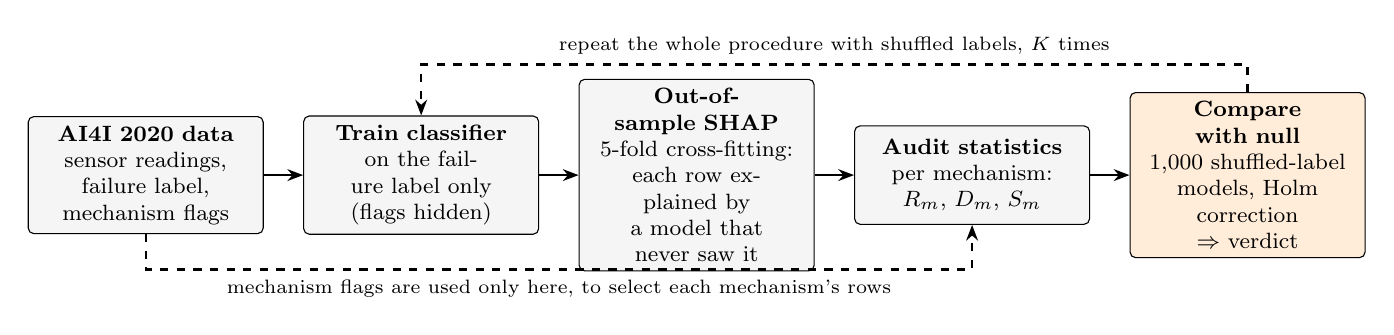
\begin{tikzpicture}[
  box/.style={draw, rounded corners=2pt, align=center, text width=2.75cm, minimum height=1.25cm,
              font=\footnotesize, fill=gray!8},
  arr/.style={-{Stealth[length=2mm]}, thick},
  node distance=0.5cm]
\node[box] (data) {\textbf{AI4I 2020 data}\\sensor readings,\\failure label,\\mechanism flags};
\node[box, right=of data] (train) {\textbf{Train classifier}\\on the failure label only\\(flags hidden)};
\node[box, right=of train] (shap) {\textbf{Out-of-sample SHAP}\\5-fold cross-fitting:\\each row explained by\\a model that never saw it};
\node[box, right=of shap] (stats) {\textbf{Audit statistics}\\per mechanism:\\$R_m$, $D_m$, $S_m$};
\node[box, right=of stats, fill=orange!15] (null) {\textbf{Compare with null}\\1{,}000 shuffled-label\\models, Holm correction\\$\Rightarrow$ verdict};
\draw[arr] (data) -- (train);
\draw[arr] (train) -- (shap);
\draw[arr] (shap) -- (stats);
\draw[arr] (stats) -- (null);
\draw[arr, dashed] (data.south) -- ++(0,-0.45) -| node[pos=0.25, below, font=\scriptsize]
  {mechanism flags are used only here, to select each mechanism's rows} (stats.south);
\draw[arr, dashed] (null.north) -- ++(0,0.35) -| node[pos=0.25, above, font=\scriptsize]
  {repeat the whole procedure with shuffled labels, $K$ times} (train.north);
\end{tikzpicture}
\caption{Overview of the audit. The model never sees the mechanism flags. The flags only decide which
rows each audit statistic looks at. The same pipeline, rerun on shuffled labels, tells us how large
each statistic would be for a model that learned nothing about failure.}
\label{fig:pipeline}
\end{figure*}

% Research questions, stated as hypotheses, with short answers
We frame the study around three hypotheses. \Cref{tab:questions} states them and gives our short
answers, which the rest of the paper supports.

\begin{table}[t]
\centering
\caption{Hypotheses tested in this paper and short answers.}
\label{tab:questions}
\footnotesize
\setlength{\tabcolsep}{3pt}
\begin{tabular}{@{}L{0.6cm}L{3.5cm}L{3.7cm}@{}}
\toprule
& Hypothesis & Answer \\
\midrule
H1 & For each physical mechanism, the model's SHAP credit falls on that mechanism's trigger features,
  more than chance would allow and more than on other failures. &
  \textbf{Yes} for heat dissipation, power, and overstrain failure, in all seeds and with two
  explainers and two model families. \textbf{Unresolved} for tool wear failure, whose result depends
  on the explainer. \\
\addlinespace
H2 & The audit catches a model that relies on a shortcut sensor. &
  \textbf{Yes}, once the shortcut takes about a fifth to a third of the credit. \textbf{No} for a
  shortcut that takes about a tenth. Accuracy does not reveal the shortcut. \\
\addlinespace
H3 & A retrained null is necessary: a baseline that compares random failure rows under the same
  model cannot tell a trained model from a shuffled-label one. &
  \textbf{Yes.} The same-model baseline approves both models. \\
\bottomrule
\end{tabular}
\end{table}

% Contributions
Our main contributions are:
\begin{enumerate}
  \item \textbf{A per-mechanism audit of SHAP explanations.} It combines three simple statistics,
    out-of-sample SHAP values, a shuffled-label null, and correction for multiple tests
    (\cref{sec:method}).
  \item \textbf{Evidence that a simple baseline is misleading.} Comparing random failure rows under
    the same model approves a model that learned nothing (\cref{sec:naive}).
  \item \textbf{Controlled stress tests.} We inject a shortcut sensor of graded strength
    (\cref{sec:sweep}), and we vary the seed, the rows audited, the features, the explainer, and the
    model family (\cref{sec:robust,sec:variants}).
  \item \textbf{A scaling study.} On data generated from the AI4I~2020 process with up to
    $3 \cdot 10^5$ rows, we show how the power of each test changes with data size; the audit's runs
    are independent, so its cost grows roughly linearly and spreads across machines
    (\cref{sec:scale}).
  \item \textbf{A comparison with simpler audit designs.} Only the full audit rejects a model trained
    on shuffled labels, avoids optimistic verdicts, and still detects a strong shortcut at 300{,}000
    rows (\cref{sec:compare}).
  \item \textbf{A reproducible benchmark} of seven model families with confidence intervals, and code
    that regenerates every number, table, and figure.
\end{enumerate}
SHAP, oversampling, and shuffled-label nulls~\cite{altmann2010permutation} are existing tools. What is
new is their use per failure mechanism, the shortcut score, and the finding that the natural
same-model baseline is fooled by how unusual mechanism rows are.

%======================================================================
\section{Related Work and Background}
\label{sec:related}

% Section intro
This section reviews three lines of prior work:
explaining models on AI4I~2020, evaluating explanations against a known answer, and randomization
tests. \Cref{tab:related} summarizes what each line of work does, what it cannot answer, and how our
audit fills that gap.

\begin{table*}[t]
\centering
\caption{Prior lines of research, what they test, and how our audit differs.}
\label{tab:related}
\footnotesize
\setlength{\tabcolsep}{4pt}
\begin{tabular}{@{}L{3.3cm}L{2.2cm}L{2.4cm}L{4.1cm}L{4.6cm}@{}}
\toprule
Line of work & What is tested & Reference answer & Limitation for our question & What our audit adds \\
\midrule
XAI on AI4I~2020~\cite{matzka2020explainable,milling2025shap} & the model & none & reports
  explanations but gives no pass/fail test & a pass/fail test per failure mechanism \\
\addlinespace
Synthetic benchmarks~\cite{liu2021synthetic,agarwal2022openxai,yang2019bam} & the explainer &
  built into synthetic data & checks whether the explainer is accurate, not whether the model is
  right & tests the model, using an exact explainer for tree models \\
\addlinespace
Feature removal~\cite{hooker2019roar,rong2022road} & the explainer & none & measures accuracy loss,
  with no link to physical causes & compares credit with the physical trigger features \\
\addlinespace
Randomization checks~\cite{adebayo2018sanity,altmann2010permutation} & the explainer or global
  importance & none & global, so it cannot say which feature explains which failure type & applies
  the shuffled-label idea to each mechanism's rows separately \\
\addlinespace
Causal PdM~\cite{causalbenchmark2026} & causal vs.\ correlational models & assumed causal graph &
  attribution comes from a new causal model, not the model in use & keeps the usual model and tests
  its explanation \\
\bottomrule
\end{tabular}
\end{table*}

\subsection{Prior Work}
\label{sec:prior}

% Explanations on AI4I: reported, not tested
\textit{Explanations on AI4I~2020.} Matzka~\cite{matzka2020explainable} introduced the dataset with
local explanations of single predictions, and Zhao et al.~\cite{milling2025shap} report global SHAP
importance for tree ensembles on it. Neither checks the explanations against the mechanism flags or
defines when an explanation counts as correct. For accuracy, Su and Tseng~\cite{physicsinformed2026}
report a positive-class F1 of 0.722 for a random forest; Khemani and
Qureshi~\cite{connectedvehicles2026} report a LightGBM ROC-AUC of 0.973 under 5-fold cross-validation
as part of a study on connected vehicles.

% Ground-truth benchmarks test explainers
\textit{Evaluating explainers against a known answer.} XAI-Bench~\cite{liu2021synthetic},
OpenXAI~\cite{agarwal2022openxai}, BAM~\cite{yang2019bam}, Zhou et al.~\cite{zhou2022attribute}, and
CLEVR-XAI~\cite{arras2022clevr} build data in which the important features are known, and
ROAR~\cite{hooker2019roar} and ROAD~\cite{rong2022road} remove top-ranked features and measure the
drop in accuracy. All of them ask whether an \emph{explainer} reports what the model uses. We ask the
reverse: given an exact explainer, does the \emph{model} use what the physical process uses? In the
terms of Chen et al.~\cite{chen2020true}, we test whether explanations are ``true to the data'' for
each failure type.

% Randomization tests: borrowed and applied per mechanism
\textit{Randomization tests.} Retraining on shuffled labels is a standard check of whether accuracy
\cite{ojala2010permutation} or feature importance~\cite{altmann2010permutation} beats chance, and
Adebayo et al.~\cite{adebayo2018sanity} used model randomization to expose saliency maps that ignore
the model (see also~\cite{kindermans2019unreliability,yona2021revisiting}). We adopt the
shuffled-label null of Altmann et al., but apply it to each mechanism's rows rather than to global
importance.

% Causal PdM: replace vs. test
\textit{Causal PdM.} Dhande et al.~\cite{causalbenchmark2026} benchmark correlational models against
a Bayesian structural causal model on data similar to AI4I~2020 and find that the causal model
attributes HDF, PWF, and OSF failures correctly. We instead keep the kind of model most PdM work
uses~\cite{serradilla2022deep} and test its explanation.

\subsection{SHAP and Its Limits}
\label{sec:shap}

% Intuition and definition
SHAP is based on the Shapley value from cooperative game theory, which splits a team's payout fairly
among players by averaging each player's added value over all orders in which they could join. SHAP
treats the features as players and the prediction as the payout~\cite{lundberg2017shap}. For a model
$f$ and input $x$ with $d$ features, it assigns each feature $j$ a value $\phi_j(x)$ such that
$f(x) = \phi_0 + \sum_{j=1}^{d} \phi_j(x)$, where $\phi_0$ is the average output. A positive value
pushes the prediction toward failure, a negative one away from it; we use the magnitude $|\phi_j(x)|$
as the size of the contribution.

% TreeSHAP variants and why we test both
TreeSHAP computes these values exactly for tree ensembles such as XGBoost and random
forests~\cite{lundberg2020treeshap}. It must evaluate the model as if some features were unknown. The
default \emph{path-dependent} version follows both branches of a split on an unknown feature, weighted
by the training rows that went each way; the \emph{interventional} version substitutes values from a
background sample of real rows, which breaks correlations between features. The two can disagree
when features are correlated~\cite{aas2021explaining}, as our derived features are, and SHAP values
depend on how missing features are modeled~\cite{janzing2020feature,kumar2020problems} and can be
manipulated~\cite{slack2020fooling}. We therefore repeat the audit with both versions
(\cref{sec:variants}).

%======================================================================
\section{Methodology}
\label{sec:method}

\subsection{Problem Setting}
\label{sec:background}

% Formal setup in plain terms
Each row of the data has a sensor vector $x_i$, a binary failure label $y_i$, and a vector $z_i$ of
mechanism flags. The model sees only $(x_i, y_i)$. For each mechanism $m$, domain knowledge gives a
set $E_m$ of \emph{trigger features}, the sensors its physical rule depends on. The audit then asks a
simple question: on the rows where mechanism $m$ occurred, does the model's SHAP credit go to $E_m$,
and more so than on other failures? We write $S_m = \{i : z_{i,m} = 1\}$ for the rows of
mechanism $m$, $F = \{i : y_i = 1\}$ for all failure rows, and $\phi_j(x_i)$ for the SHAP value of
feature $j$ on row $i$.

\subsection{Dataset and Failure Mechanisms}
\label{sec:data}

% Dataset contents and imbalance
AI4I~2020~\cite{matzka2020explainable} contains 10{,}000 rows from a simulated milling process. Each
row has a product quality type (\texttt{L}, \texttt{M}, or \texttt{H}), five process variables (air
temperature, process temperature, rotational speed, torque, and tool wear), the failure label, and
five mechanism flags. Only 339 rows (3.4\%) are failures, so the classes are highly imbalanced.

% The five mechanisms
The failure label is the logical OR of five mechanisms, listed in \cref{tab:mechanisms}. Four of them
follow published rules on the sensor values. The fifth, random failure (RNF), happens with a small
fixed probability and has no trigger features, so we treat it only descriptively.

\begin{table}[t]
\centering
\caption{Failure mechanisms in AI4I~2020~\cite{matzka2020explainable}, their trigger rules, and the
trigger features $E_m$ used by the audit. Counts are as released. The TWF failure point is random
within the window.}
\label{tab:mechanisms}
\footnotesize
\setlength{\tabcolsep}{3pt}
\begin{tabular}{@{}lL{3.4cm}L{2.9cm}r@{}}
\toprule
Mech. & Trigger & $E_m$ & $n$ \\
\midrule
TWF & tool wear at a random point in 200--240\,min & tool wear & 46 \\
HDF & (process $-$ air temp.) $< 8.6$\,K and speed $< 1380$\,rpm & both temps., their difference,
  speed & 115 \\
PWF & torque $\times$ speed (rad/s) outside [3500, 9000]\,W & torque, speed, power & 95 \\
OSF & tool wear $\times$ torque above 11{,}000/\allowbreak 12{,}000/\allowbreak 13{,}000\,min$\cdot$Nm for L/M/H & tool
  wear, torque, overstrain, its ratio & 98 \\
RNF & 0.1\% chance, independent of the process & -- & 19 \\
\bottomrule
\end{tabular}
\end{table}

% Label inconsistencies
The released labels do not follow the OR rule exactly: 24 rows carry several flags, 9 failures carry
none, and 18 of the 19 RNF rows are not marked as failures. We therefore audit all flagged rows and,
as a check, only the rows with exactly one flag.

\subsection{Features}
\label{sec:features}

% Derived features and why
The trigger rules combine raw sensors, so we add four derived features computed from the raw values,
not from the flags: \emph{power} (torque $\times$ speed), \emph{temperature difference} (process
$-$ air), \emph{overstrain} (tool wear $\times$ torque), and \emph{overstrain ratio} (overstrain
divided by the type-specific limit). The mechanism flags are parts of the label, so they are never
used as inputs.

% Circularity: why a simulator, and why the result is not built in
\textit{Is the audit circular?} AI4I~2020 is simulated, and its labels come from the same rules we
audit against. We use it because real maintenance data rarely records the cause of each failure, so
an audit can only be validated where the causes are known. A simulator does not make the result
automatic: a model can still fit the label through shortcuts or other features, and the audit
rejects the shuffled-label model, flags an injected shortcut, and refuses to pass tool wear failure.
Because the derived features could still make the audit easier, we also repeat it with raw features
only (\cref{sec:robust}).

\subsection{Audit Statistics}
\label{sec:stats}

% Share of credit on the trigger features
For a set of rows $S$ and a mechanism $m$, let $I_{m,j}(S) = |S|^{-1} \sum_{i \in S}
|\phi_j(x_i)|$ be the average SHAP magnitude of feature $j$ on those rows. The share of credit that
goes to the trigger features is
\begin{equation}
  r_m(S) = \sum_{j \in E_m} I_{m,j}(S) \Big/ \sum_{j=1}^{d} I_{m,j}(S).
\end{equation}

% Three statistics
From this we build three statistics:
\begin{align}
  R_m &= r_m(S_m), \label{eq:share} \\
  D_m &= r_m(S_m) - r_m(F \setminus S_m), \label{eq:spec} \\
  S_m &= \max_{j \notin E_m} \big[ s_j(S_m) - s_j(F \setminus S_m) \big], \label{eq:shortcut}
\end{align}
where $s_j(S) = I_{m,j}(S) / \sum_{k} I_{m,k}(S)$ is the share of a single feature $j$.
\Cref{tab:stats} explains what each statistic asks and when a mechanism passes.

\begin{table}[t]
\centering
\caption{The three audit statistics in plain terms. A mechanism passes the audit when $R_m$ and $D_m$
are significantly larger than under the null and $S_m$ is not.}
\label{tab:stats}
\footnotesize
\setlength{\tabcolsep}{3pt}
\begin{tabular}{@{}L{1.85cm}L{4.1cm}L{1.6cm}@{}}
\toprule
Statistic & Question it answers & Pass if \\
\midrule
$R_m$, relevant share & On this mechanism's rows, how much of the credit goes to its trigger
  features? & large \\
$D_m$, specificity & Is that share larger on this mechanism's rows than on other failures? &
  large \\
$S_m$, shortcut score & Does some \emph{other} feature gain credit specifically on this mechanism's
  rows? & not large \\
\bottomrule
\end{tabular}
\end{table}

% Worked example
\textit{Worked example.} On the 95 power failure (PWF) rows, the average SHAP magnitudes of the
three PWF trigger features are 4.96 (power), 1.93 (torque), and 1.33 (speed), which sum to 8.22. The
twelve input features together sum to 11.82 (\cref{fig:shap}a). Hence
$R_{\mathrm{PWF}} = 8.22 / 11.82 \approx 0.70$: about 70\% of the model's credit on power failures
goes to the features that physically cause them. Whether 70\% is ``high'' is decided by the null in
\cref{sec:nulls}, not by eye.

% Why three
Each statistic covers a gap in the others. $R_m$ alone can be high simply because the trigger
features matter for all failures; $D_m$ checks that the credit is specific to this mechanism. Both
can still be high while a non-trigger feature also takes a large share; $S_m$ catches this case,
which is what a shortcut looks like. $S_m$ is related to conditional randomization and knockoff
tests~\cite{candes2018panning}, but it is computed from the explanation and only on the mechanism's
rows.

\subsection{Out-of-Sample Explanations}
\label{sec:oos}

% Cross-fitting
SHAP values computed on training rows describe what the model memorized about those rows, not what
it learned in general. A model can fit its training failures closely and still explain new failures
poorly. We therefore use cross-fitting~\cite{chernozhukov2018double}. We split the data into five
folds of equal size, each with the same failure rate (\emph{stratified}). For each fold, we train the
full pipeline on the other four folds and compute SHAP values on the held-out fold. After five
rounds, every row has a SHAP value from a model that never saw it during training, and the audit uses
only these values. \Cref{sec:robust} shows that skipping this step changes the result.

\subsection{Choosing the Right Null}
\label{sec:nulls}

% The naive null and why it fails
\textit{Naive null.} The obvious test compares $R_m$ with the same statistic on random failure rows
of equal size under the same model. This test is flawed. Rows of a mechanism are selected by extreme
values of its trigger features, and SHAP values tend to be large at extreme values even for a model
that learned nothing. We confirm this in \cref{sec:naive}.

% The model-randomization null: what shuffling does
\textit{Shuffled-label null.} We instead compare the real model with models that cannot know
anything about failure. To build one, we randomly reorder the failure labels across rows. This keeps
the sensor values, the failure rate, and the whole training pipeline unchanged, but it destroys any
real link between the sensors and failure. The mechanism flags stay attached to their rows, so the
audit still looks at the same rows. We then rerun the full procedure (features, oversampling,
training, and cross-fitting) on the shuffled labels, keeping the hyperparameters tuned on the real
labels, and compute all three statistics. Repeating this $K$ times gives $K$ values of each statistic
that show how large it can be by chance, including the effect of unusual feature values that breaks
the naive null.

% p-value
For a statistic $T$ of the real model with null values $T^{(1)}, \dots, T^{(K)}$, the $p$-value is
\begin{equation}
  p = \frac{1 + \#\{k : T^{(k)} \ge T\}}{K + 1},
\end{equation}
the fraction of null models that score at least as high as the real model, counting the real model
once so that $p$ is never zero. With $K = 1{,}000$, the smallest possible value is
$1/1{,}001 \approx 0.001$, reached when no null model scores as high as the real one.

% Holm correction
Because we test four mechanisms, one could pass by chance. Holm's method~\cite{holm1979simple}
guards against this: it sorts the four $p$-values, multiplies the smallest by 4, the next by 3, and so
on, which keeps the chance of any false pass below 5\%. A mechanism passes a test if its adjusted
$p$ is below 0.05; for example, an unadjusted 0.001 becomes 0.004 (\cref{tab:audit}).

% RNF
\textit{Random failures.} RNF has no trigger features. We only report whether its credit is more
concentrated on a single feature than under the null.

\subsection{Model Training and Selection}
\label{sec:training}

% Split and oversampling
We split the data 70/20/10 into training, validation, and test sets, stratified by label, and fit
scaling and one-hot encoding on the training set only, so that no information from the validation
or test rows leaks into training.

% Oversampling, explained
With only 3.4\% failures, a model can reach 96.6\% accuracy by never predicting failure, so we
\emph{oversample} the failure class in the training data. SMOTE~\cite{chawla2002smote}
creates a synthetic failure row by picking a real failure row and moving it part of the way toward
one of its nearest failure neighbors. Borderline-SMOTE~\cite{han2005borderline} does this only for
failure rows that lie close to non-failure rows, where the model is most likely to make mistakes.
ADASYN~\cite{he2008adasyn} creates more synthetic rows where failures are hardest to learn. We
compare the three using the validation F1 of a default XGBoost~\cite{chen2016xgboost} model and keep
the best (\cref{sec:perf}).

% Model families
We train seven model families: logistic regression, a support vector machine (SVM) with a radial
basis function kernel, $k$-nearest neighbors ($k$-NN, $k = 7$), a decision tree (depth 10), a random
forest (300 trees, depth 12), XGBoost (300 trees, depth 6, learning rate 0.1), and a multilayer
perceptron (MLP) with hidden layers of 64 and 32 units. Other hyperparameters are library defaults
(scikit-learn 1.9.1, XGBoost 3.4.1, PyTorch 2.14.0), and the random seed is 42.

% Tuning and thresholds
XGBoost has the highest validation F1, so we tune it with a 40-iteration randomized search under
5-fold stratified cross-validation, scored on F1. Borderline-SMOTE runs inside the search pipeline,
so each fold oversamples only its own training part. The search covers depth 3--8, 200--600 trees,
learning rate 0.01--0.2, row and column subsampling 0.6--1.0, minimum child weight 1--5, and $\gamma$
0--0.3. The model outputs a failure probability for each row, and a row raises an alarm when this
probability exceeds a \emph{decision threshold}. We choose the threshold that maximizes F1 on the
validation set.

% Metrics, explained
\textit{Evaluation metrics.} Because failures are rare, we report metrics for the failure class.
\emph{Precision} is the share of alarms that are real failures, \emph{recall} the share of real
failures that raise an alarm, and \emph{F1} their harmonic mean. \emph{ROC-AUC} measures how well the
model ranks failures above non-failures over all thresholds. The \emph{Brier score} (mean squared
error of the predicted probability) and the \emph{expected calibration error} (ECE, the average gap
between predicted and observed failure rates) check whether probabilities can be taken at face
value; lower is better for both.

% Uncertainty
A small test set makes every metric uncertain, so we report 95\% confidence intervals (CIs): exact
binomial (Clopper--Pearson) intervals for precision and recall, and intervals from 5{,}000 stratified
bootstrap resamples of the test set otherwise. We also run 5-fold cross-validation of the whole
pipeline at a threshold of 0.5. The hyperparameters are tuned on the training split that this
cross-validation reuses, so its F1 is slightly optimistic.

\subsection{Experimental Plan}
\label{sec:setup}

% One table for all experiments
\Cref{tab:plan} lists every experiment, the question it answers, and the number $K$ of
shuffled-label models in its null. The primary audit uses $K = 1{,}000$, so the smallest possible
$p$-value before correction is 0.001; it takes 12 minutes on eight CPU cores.

\begin{table}[t]
\centering
\caption{Experimental plan.}
\label{tab:plan}
\footnotesize
\setlength{\tabcolsep}{3pt}
\begin{tabular}{@{}L{2.55cm}L{3.75cm}r@{}}
\toprule
Experiment & Question & $K$ \\
\midrule
Primary audit, seed 42 & Do the explanations match each mechanism? (H1) & 1{,}000 \\
Seeds 1--4 & Is the result stable across seeds? & 200 \\
Single-flag rows & Do rows with several flags change the result? & 1{,}000 \\
Raw features only & Do the derived features make the audit circular? & 1{,}000 \\
In-sample SHAP & Does explaining training rows inflate the result? & 1{,}000 \\
Interventional TreeSHAP & Does the result depend on the explainer? & 200 \\
Random forest & Does it depend on the model family? & 200 \\
Shuffled-label model & Sanity check; does the naive null fail? (H3) & 200 \\
Shortcut sweep & When is an injected shortcut caught? (H2) & 500 \\
Scaling, $10^4$--$3 \cdot 10^5$ rows & How do power and cost change with size? & 200 \\
\bottomrule
\end{tabular}
\end{table}

% Explainer variant details
\textit{Explainer and model variants.} The interventional runs use backgrounds of 100, 500, and
1{,}000 training rows per fold; their null runs use the same explainer, and the random-forest null
uses the random forest.

% Shortcut sensor
\textit{Shortcut sensor.} To test H2, we add a fake sensor $s = z_{\mathrm{HDF}} +
\mathcal{N}(0, \sigma^2)$, a noisy copy of the heat dissipation flag with no physical meaning, and
vary the noise $\sigma$ from 2 down to 0.1. A smaller $\sigma$ makes the sensor a stronger shortcut.
The sensor is not in $E_{\mathrm{HDF}}$, so a model that relies on it should fail the HDF audit.

% Sanity model
\textit{Shuffled-label model.} A model trained on shuffled labels is interchangeable with the null
runs, so we use it only as a check of the code and as the case the naive null should reject.

% Data generator for scaling
\textit{Generated data for scaling.} To study larger data, we generate new rows from the process
documented with AI4I~2020~\cite{matzka2020explainable}, copying no released row. The sensor
distributions follow the documentation and the release; tool wear grows until the tool reaches a
life drawn from $U(200, 240)$\,min, where it fails (TWF) with probability 0.4; and HDF, PWF, and OSF
follow the published rules, which reproduce the released flags exactly. The generated failure rate is
3.5--4.0\%, against 3.4\% in the release. We audit $n \in \{10^4, 3 \cdot 10^4, 10^5\}$ with three
generation seeds and $3 \cdot 10^5$ with one, each without the shortcut sensor and with it at
$\sigma \in \{0.35, 0.25\}$. The full generator is in the released code.

%======================================================================
\section{Results}
\label{sec:results}

\subsection{Predictive Performance}
\label{sec:perf}

% Oversampler choice
\textit{Oversampler.} On the validation set, Borderline-SMOTE gives the highest F1 (0.826, against
0.768 for SMOTE and 0.747 for ADASYN). The other two reach slightly higher recall but lose more
precision, so we use Borderline-SMOTE in all later experiments.

% Model comparison
\textit{Model comparison.} \Cref{tab:models} reports test results for all models. Tree ensembles
clearly outperform the linear and distance-based models. The tuned XGBoost reaches F1 0.89 at its
validation-selected threshold of 0.978, against 0.87 for the default XGBoost at 0.5. The confidence
intervals overlap, so we cannot claim that tuning or the threshold helps.

\begin{table}[t]
\centering
\caption{Failure-class test metrics, sorted by F1, with bootstrap 95\% CI for F1. ROC-AUC: area
under the receiver operating characteristic curve.}
\label{tab:models}
\footnotesize
\setlength{\tabcolsep}{4pt}
\begin{tabular}{@{}lrrlr@{}}
\toprule
Model & Prec. & Rec. & F1 (95\% CI) & ROC-AUC \\
\midrule
XGBoost (tuned) & \textbf{1.00} & 0.79 & \textbf{0.89} (0.79--0.95) & 0.988 \\
XGBoost & 0.86 & 0.88 & 0.87 (0.78--0.94) & 0.988 \\
Random forest & 0.79 & 0.88 & 0.83 (0.74--0.92) & \textbf{0.989} \\
MLP & 0.65 & \textbf{0.91} & 0.76 (0.67--0.84) & 0.988 \\
Decision tree & 0.68 & 0.82 & 0.75 (0.64--0.84) & 0.927 \\
SVM & 0.42 & 0.88 & 0.57 (0.48--0.65) & 0.976 \\
k-NN & 0.43 & 0.79 & 0.56 (0.46--0.65) & 0.877 \\
Logistic regression & 0.24 & 0.85 & 0.37 (0.31--0.43) & 0.943 \\
\bottomrule
\end{tabular}

\end{table}

% Uncertainty and calibration
\textit{Uncertainty.} The test set holds only 34 failures, so the intervals are wide. The tuned model
raises 27 alarms, all of them real failures, and misses 7 failures. This gives precision 1.00 (95\% CI
0.87--1.00) and recall 0.79 (0.62--0.91). Its probabilities are well calibrated: the Brier score is
0.0090, against 0.033 for always predicting the base rate, and the expected calibration error is
0.008.

% Comparison with prior work
\textit{Comparison with prior work.} Five-fold cross-validation of the full pipeline gives a
failure-class F1 of $0.822 \pm 0.013$ and a macro-F1 of $0.908 \pm 0.007$. Both this and our
single-split F1 of 0.89 are above the 0.722 reported by Su and Tseng~\cite{physicsinformed2026} on the
same binary task. The model is therefore accurate enough to be a realistic target for the audit.

\subsection{Main Audit of the Tuned Model (H1)}
\label{sec:audit-results}

% How to read the overview figure
\Cref{fig:overview} is the central result of the paper. Each gray dot is one of the 1{,}000 models
trained on shuffled labels; together they show how large $R_m$ and $D_m$ can be by chance. The orange
dot is the real model. A mechanism passes when the orange dot sits clearly above the gray cloud.

\begin{figure}[t]
\centering
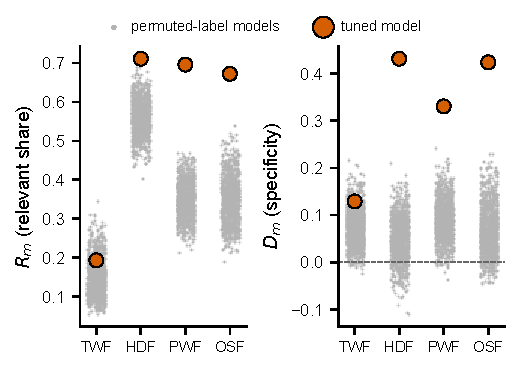
\includegraphics[width=\columnwidth]{audit_overview.pdf}
\caption{Main audit. Out-of-sample relevant share $R_m$ (left) and specificity $D_m$ (right) of the
tuned model (orange) against 1{,}000 shuffled-label models (gray). For HDF, PWF, and OSF the real
model lies above every null model on both statistics. For TWF it lies inside the null cloud.}
\label{fig:overview}
\end{figure}

% Three mechanisms pass
\textit{Heat dissipation, power, and overstrain failure pass.} For these three mechanisms the real
model lies above every shuffled-label model on both statistics, and all adjusted $p$-values are
0.004 (\cref{tab:audit}). On their rows, the share of credit on the trigger features exceeds the
share on other failures by 0.33 to 0.43, while the null averages stay below 0.09. The shortcut score
flags nothing, and the top feature of each mechanism is one of its trigger features.

\begin{table*}[t]
\centering
\caption{Main audit (cross-fitted, seed 42, $K = 1{,}000$). Null: mean over shuffled-label models.
$p$: Holm-adjusted over the four physical mechanisms; $^{\times}$ marks a failed $R_m$ or $D_m$ test
($p \ge 0.05$); $S_m$ (\cref{eq:shortcut}) flags a shortcut if $p < 0.05$. For RNF the statistic is
the largest feature's share, and $p$ tests for more concentration than the null.}
\label{tab:audit}
\footnotesize
\begin{tabular}{@{}lrlrrrrrrrrr@{}}
\toprule
& $n$ & Top feature & $R_m$ & Null & $p$ & $D_m$ & Null & $p$ & $S_m$ & Null & $p$ \\
\midrule
TWF & 46 & tool wear & 0.193 & 0.152 & 0.201$^{\times}$ & 0.129 & 0.070 & 0.077$^{\times}$ & 0.025 & 0.025 & 1.000 \\
HDF & 115 & speed & 0.711 & 0.557 & 0.004 & 0.431 & 0.049 & 0.004 & 0.001 & 0.015 & 1.000 \\
PWF & 95 & power & 0.696 & 0.347 & 0.004 & 0.330 & 0.088 & 0.004 & 0.001 & 0.011 & 1.000 \\
OSF & 98 & overstrain ratio & 0.672 & 0.345 & 0.004 & 0.424 & 0.067 & 0.004 & -0.001 & 0.019 & 1.000 \\
RNF & 19 & speed & 0.186 & 0.240 & 0.985 & -- & -- & -- & -- & -- & -- \\
\bottomrule
\end{tabular}

\end{table*}

% TWF fails
\textit{Tool wear failure does not pass.} TWF fails both tests ($p = 0.201$ and $0.077$). Tool wear
is still its top feature, but it takes only 19\% of the credit on TWF rows, against 15\% under the
null. This is not surprising: the TWF rule fires at a \emph{random} point inside a tool-wear window,
so tool wear only partly determines it, and 46 rows give the model little to learn from.

% What the heatmap shows vs. the global plot
\Cref{fig:shap} shows why a per-mechanism view is needed. The heatmap (a) shows the average SHAP
magnitude of each feature on each mechanism's rows. Each physical mechanism lights up its own
trigger features: speed and temperature difference for HDF, power and torque for PWF, and the
overstrain ratio for OSF. The usual global summary (b) ranks speed, power, and tool wear highest
overall, but it mixes all failures together and cannot tell which feature explains which failure.

\begin{figure*}[t]
\centering
\begin{minipage}[b]{0.49\textwidth}
\centering
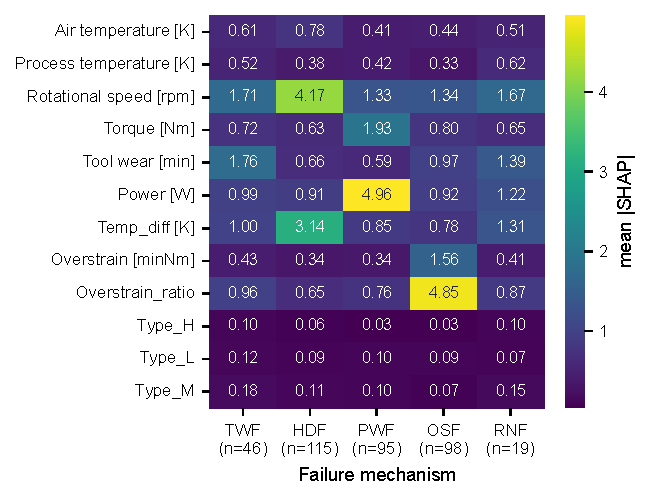
\includegraphics[width=0.93\linewidth,height=5.2cm,keepaspectratio]{shap_crosscheck_heatmap.pdf}\\
\small (a) Mean out-of-sample $|\phi_j|$ on the rows of each mechanism
\end{minipage}\hfill
\begin{minipage}[b]{0.47\textwidth}
\centering
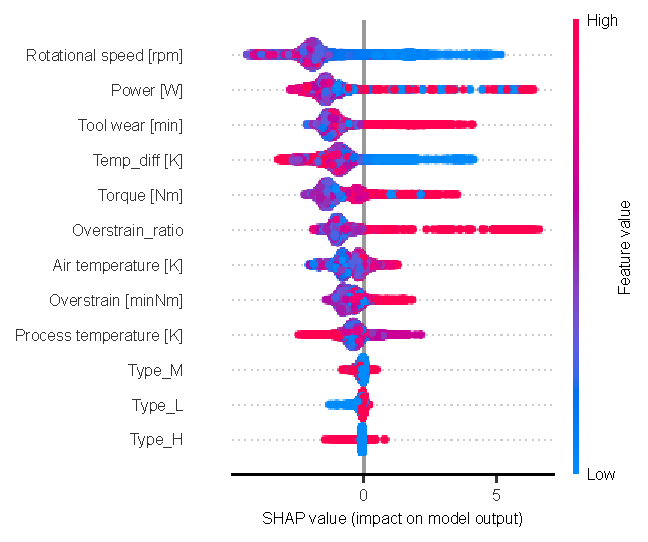
\includegraphics[width=0.93\linewidth,height=5.2cm,keepaspectratio]{shap_summary.pdf}\\
\small (b) Global SHAP summary on all rows
\end{minipage}
\caption{SHAP explanations of the tuned model. (a) Per-mechanism view used by the audit: each
mechanism's credit concentrates on its own trigger features (bright cells). (b) The standard global
view ranks features overall but does not separate the mechanisms.}
\label{fig:shap}
\end{figure*}

%======================================================================
\section{Experimental Analysis}
\label{sec:analysis}

% Section intro
We now change the choices behind the main audit one at a time, test the naive baseline, inject a
shortcut, and scale up the data. \Cref{tab:robust} collects the $p$-values of all variants.

\begin{table*}[t]
\centering
\caption{Holm-adjusted audit $p$-values for $R_m$, $D_m$, and $S_m$ across analysis variants.
$^{\times}$ marks a failed $R$ or $D$ test ($p \ge 0.05$) and $^{\dagger}$ a flagged shortcut
($p_S < 0.05$); no variant flags one. Interventional rows use background seed 0; seeds 1 and 2 give
the same verdicts. The smallest attainable adjusted $p$ is $4/(K+1)$. The shuffled-label model is
interchangeable with its null and serves only as a sanity check; the last two rows apply the naive
null of \cref{sec:nulls}.}
\label{tab:robust}
\footnotesize
\setlength{\tabcolsep}{3.2pt}
\begin{tabular}{@{}lrrrrrrrrrrrrr@{}}
\toprule
& & \multicolumn{3}{c}{TWF} & \multicolumn{3}{c}{HDF} & \multicolumn{3}{c}{PWF} & \multicolumn{3}{c}{OSF} \\
\cmidrule(lr){3-5}\cmidrule(lr){6-8}\cmidrule(lr){9-11}\cmidrule(lr){12-14}
Variant & $K$ & $R$ & $D$ & $S$ & $R$ & $D$ & $S$ & $R$ & $D$ & $S$ & $R$ & $D$ & $S$ \\
\midrule
Primary, seed 42 & 1000 & 0.201$^{\times}$ & 0.077$^{\times}$ & 1.000 & 0.004 & 0.004 & 1.000 & 0.004 & 0.004 & 1.000 & 0.004 & 0.004 & 1.000 \\
\quad single-mechanism rows & 1000 & 0.187$^{\times}$ & 0.076$^{\times}$ & 1.000 & 0.004 & 0.004 & 1.000 & 0.004 & 0.004 & 1.000 & 0.004 & 0.004 & 1.000 \\
Seed 1 & 200 & 0.199$^{\times}$ & 0.119$^{\times}$ & 0.776 & 0.020 & 0.020 & 1.000 & 0.020 & 0.020 & 1.000 & 0.020 & 0.020 & 1.000 \\
Seed 2 & 200 & 0.149$^{\times}$ & 0.065$^{\times}$ & 0.498 & 0.020 & 0.020 & 1.000 & 0.020 & 0.020 & 1.000 & 0.020 & 0.020 & 1.000 \\
Seed 3 & 200 & 0.174$^{\times}$ & 0.095$^{\times}$ & 0.736 & 0.020 & 0.020 & 1.000 & 0.020 & 0.020 & 1.000 & 0.020 & 0.020 & 1.000 \\
Seed 4 & 200 & 0.269$^{\times}$ & 0.129$^{\times}$ & 1.000 & 0.020 & 0.020 & 1.000 & 0.020 & 0.020 & 1.000 & 0.020 & 0.020 & 1.000 \\
Raw features only & 1000 & 0.345$^{\times}$ & 0.616$^{\times}$ & 1.000 & 0.190$^{\times}$ & 0.004 & 1.000 & 0.004 & 0.004 & 1.000 & 0.004 & 0.048 & 1.000 \\
In-sample SHAP & 1000 & 0.004 & 0.004 & 1.000 & 0.004 & 0.004 & 1.000 & 0.004 & 0.004 & 1.000 & 0.004 & 0.004 & 1.000 \\
Interventional, background 100 & 200 & 0.020 & 0.020 & 1.000 & 0.020 & 0.020 & 1.000 & 0.020 & 0.020 & 1.000 & 0.020 & 0.020 & 1.000 \\
Interventional, background 500 & 200 & 0.020 & 0.020 & 1.000 & 0.020 & 0.020 & 1.000 & 0.020 & 0.020 & 1.000 & 0.020 & 0.020 & 1.000 \\
Interventional, background 1000 & 200 & 0.020 & 0.020 & 1.000 & 0.020 & 0.020 & 1.000 & 0.020 & 0.020 & 1.000 & 0.020 & 0.020 & 1.000 \\
Random forest & 200 & 0.617$^{\times}$ & 0.398$^{\times}$ & 1.000 & 0.020 & 0.020 & 1.000 & 0.020 & 0.020 & 1.000 & 0.040 & 0.020 & 1.000 \\
Permuted labels (sanity) & 200 & 1.000$^{\times}$ & 0.731$^{\times}$ & 1.000 & 0.199$^{\times}$ & 0.557$^{\times}$ & 1.000 & 1.000$^{\times}$ & 0.731$^{\times}$ & 1.000 & 1.000$^{\times}$ & 0.731$^{\times}$ & 0.637 \\
\midrule
Naive null, tuned model & -- & 0.002 & -- & -- & 0.002 & -- & -- & 0.002 & -- & -- & 0.002 & -- & -- \\
Naive null, permuted labels & -- & 0.002 & -- & -- & 0.002 & -- & -- & 0.002 & -- & -- & 0.002 & -- & -- \\
\bottomrule
\end{tabular}

\end{table*}

\subsection{Robustness of the Main Audit (H1)}
\label{sec:robust}

% Seeds and single-flag rows
\textit{Seeds and rows.} The HDF, PWF, and OSF verdicts hold in all five seeds and on rows with a
single flag. TWF fails both tests in every seed.

% In-sample SHAP
\textit{In-sample explanations.} When SHAP values come from a model that has seen every audited row,
all four mechanisms pass, including TWF ($p = 0.004$; $R_{\mathrm{TWF}} = 0.35$ against 0.19 out of
sample). In-sample explanations can therefore make a model look better aligned than it is, which is
why the audit uses cross-fitting.

% Raw features
\textit{Raw features only.} Without the derived features, PWF and OSF still pass both tests (OSF
specificity narrowly, $p = 0.048$). HDF passes only on specificity, and TWF on neither. The derived
features help the HDF verdict but are not needed for PWF and OSF, so the audit is not circular for
those two. HDF is defined by a \emph{difference} of two temperatures, which a tree model can only
approximate with many splits, so it is harder to audit from raw inputs.

\subsection{Is the Naive Null Enough? (H3)}
\label{sec:naive}

% The naive null approves a model that learned nothing
Under the shuffled-label null, the shuffled-label model fails every test, as it should. Under the
naive null, however, the same model passes on all four mechanisms (adjusted $p = 0.002$), exactly as
the real model does, and even TWF passes, which the shuffled-label null rejects. The naive null
therefore cannot tell a trained model from one that learned nothing, which supports H3: a
retrained null is necessary. Any
subgroup-level test of explanations needs a null that accounts for how unusual the audited rows are.

\subsection{Detecting an Injected Shortcut (H2)}
\label{sec:sweep}

% How to read the sweep figure
\Cref{fig:sweep} shows what happens as the fake sensor becomes a stronger shortcut (left to right):
credit moves from the real trigger features (orange) to the fake sensor (blue).

\begin{figure}[t]
\centering
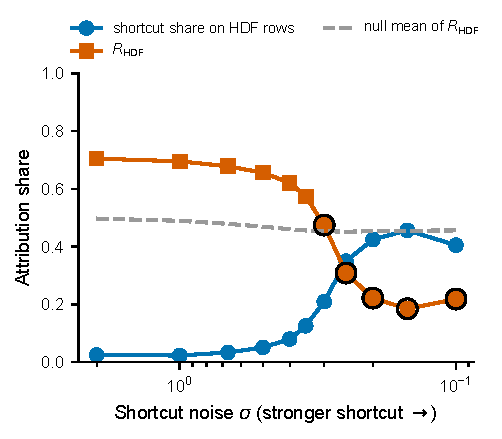
\includegraphics[width=0.95\columnwidth]{shortcut_sweep.pdf}
\caption{Shortcut sweep. As the noise $\sigma$ shrinks (left to right), the fake sensor takes more of
the credit on HDF rows (blue) and the share on the true trigger features falls (orange). Circles mark
noise levels at which the HDF relevant-share test fails.}
\label{fig:sweep}
\end{figure}

% When the audit catches the shortcut
With $K = 500$ null models, the audit's response falls into three stages:
\begin{itemize}
  \item \textbf{Weak shortcut ($\sigma \ge 0.4$).} The sensor takes at most 8\% of the credit and the
    audit passes. This is correct, because the model barely uses it.
  \item \textbf{Moderate shortcut ($\sigma = 0.35$ to $0.3$).} At 13\% the relevant-share test
    still passes narrowly ($p = 0.044$). At 21\% ($\sigma = 0.3$) it fails.
  \item \textbf{Strong shortcut ($\sigma \le 0.25$).} At 35\% the shortcut score also flags the
    sensor, and from 42\% ($\sigma = 0.2$) the specificity test fails as well.
\end{itemize}


% Accuracy hides it
Throughout the sweep, test F1 stays between 0.84 and 0.92. Accuracy alone would never reveal that
the model has started to rely on a meaningless sensor. On the released data, H2 holds once a shortcut
takes about a fifth of the credit, but not for lighter use. PWF and OSF pass at every noise level, so
the audit does not raise false alarms on unaffected mechanisms. TWF stays near the decision boundary:
its specificity test passes narrowly at four levels ($0.030 \le p \le 0.0499$) and fails at the
other seven.

% Why the shortcut score is conservative
The shortcut score is conservative here because the null models see the sensor too and give it some
credit on HDF rows, where its values are unusual (null mean of $S_{\mathrm{HDF}}$: 0.09).

\begin{table*}[t]
\centering
\caption{Comparison of audit designs on three basic checks. Each simpler design removes one
ingredient of the full audit. Values are Holm-adjusted $p$-values (HDF for check 3) or run
counts from \cref{tab:robust,tab:scale} and one additional experiment per remaining cell.}
\label{tab:compare}
\footnotesize
\setlength{\tabcolsep}{4pt}
\begin{tabular}{@{}L{5.6cm}L{3.8cm}L{3.6cm}L{3.8cm}@{}}
\toprule
Design & 1. Rejects shuffled-label model? & 2. Avoids optimism on TWF? & 3. Catches shortcut at
  $3 \cdot 10^5$ rows? \\
\midrule
Global SHAP ranking (common practice~\cite{milling2025shap}) & no verdict & no verdict & no verdict \\
Naive null (random failure rows, same model) & \textbf{No}: all pass ($p = 0.002$) & \textbf{No}:
  passes ($p = 0.002$) & \textbf{No}: HDF passes ($p = 0.002$) \\
In-sample SHAP with shuffled-label null & Yes: all fail ($p \ge 0.22$) & \textbf{No}: passes
  ($p = 0.004$) & \textbf{No}: $R$, $D$ pass; $p_S = 0.06$ \\
Relevant share $R_m$ only (out-of-sample, shuffled null) & Yes & Yes ($p = 0.201$) & \textbf{No}:
  0 of 1 runs \\
\textbf{Full audit} ($R_m$, $D_m$, $S_m$, out-of-sample, shuffled null) & \textbf{Yes}: all fail &
  \textbf{Yes}: fails ($p = 0.201$, $0.077$) & \textbf{Yes}: 1 of 1 runs \\
\bottomrule
\end{tabular}
\end{table*}

\subsection{Explainer and Model Variants}
\label{sec:variants}

% HDF/PWF/OSF stable; TWF depends on explainer
The HDF, PWF, and OSF verdicts hold with interventional TreeSHAP and with a random forest
(\cref{tab:robust}). TWF does not behave consistently. With interventional TreeSHAP it passes both
tests at every background size and seed ($R_{\mathrm{TWF}}$ between 0.45 and 0.47, tool wear its top
feature). With the random forest it fails both ($R_{\mathrm{TWF}} = 0.13$, speed its top feature).

% Why
A likely reason is correlation. Tool wear has a Spearman correlation of 0.92 with both overstrain
features, so they almost always rise and fall together. Path-dependent TreeSHAP spreads credit over features correlated with the ones a tree
splits on, while the interventional version breaks that dependence~\cite{aas2021explaining}. An
audit verdict is therefore a statement about a model \emph{and} an explainer together. A mechanism
that passes under only one explainer should be reported as unresolved.

\subsection{Scaling to Larger Data (H1, H2)}
\label{sec:scale}

% True mechanisms stay stable
\Cref{tab:scale} repeats the audit on generated data of increasing size. Without the shortcut
sensor, HDF, PWF, and OSF pass both tests and are never flagged at any size or seed. TWF fails the
relevant-share test in every run, so more data alone does not resolve it. The shortcut score flags
TWF in 3 of 10 runs without the sensor, each time for process temperature, which plays no role in
tool wear failure; the effect is small ($S_{\mathrm{TWF}} \le 0.05$).

\begin{table}[t]
\centering
\caption{Audit on data generated from the AI4I~2020 process at size $n$ ($K = 200$): mean sensor
share of the HDF credit, and the fraction of generation seeds in which the HDF shortcut is flagged by
the relevant-share test ($p_R \ge 0.05$) or the shortcut score ($p_S < 0.05$), TWF passes the
specificity test, or the shortcut score flags TWF. Min.: wall-clock minutes for one audit on eight
cores. HDF, PWF, and OSF pass the $R$ and $D$ tests in every run without the sensor.}
\label{tab:scale}
\footnotesize
\setlength{\tabcolsep}{3pt}
\begin{tabular}{@{}rlrrrrrrr@{}}
\toprule
& & & & \multicolumn{2}{c}{HDF flagged by} & \multicolumn{2}{c}{TWF} & \\
\cmidrule(lr){5-6}\cmidrule(lr){7-8}
$n$ & $\sigma$ & Seeds & Sensor & $R$ & $S$ & $D$ pass & $S$ flag & Min. \\
\midrule
10{,}000 & -- & 3 & 0.000 & 0/3 & 0/3 & 0/3 & 0/3 & 3 \\
 & 0.35 & 3 & 0.158 & 2/3 & 0/3 & 0/3 & 0/3 & 3 \\
 & 0.25 & 3 & 0.390 & 3/3 & 3/3 & 0/3 & 0/3 & 3 \\
30{,}000 & -- & 3 & 0.000 & 0/3 & 0/3 & 0/3 & 1/3 & 7 \\
 & 0.35 & 3 & 0.128 & 0/3 & 0/3 & 2/3 & 0/3 & 6 \\
 & 0.25 & 3 & 0.346 & 3/3 & 3/3 & 2/3 & 1/3 & 7 \\
100{,}000 & -- & 3 & 0.000 & 0/3 & 0/3 & 1/3 & 2/3 & 17 \\
 & 0.35 & 3 & 0.100 & 0/3 & 0/3 & 2/3 & 1/3 & 19 \\
 & 0.25 & 3 & 0.315 & 3/3 & 3/3 & 2/3 & 1/3 & 19 \\
300{,}000 & -- & 1 & 0.000 & 0/1 & 0/1 & 0/1 & 0/1 & 52 \\
 & 0.35 & 1 & 0.063 & 0/1 & 0/1 & 0/1 & 0/1 & 59 \\
 & 0.25 & 1 & 0.271 & 0/1 & 1/1 & 0/1 & 1/1 & 61 \\
\bottomrule
\end{tabular}

\end{table}

% The two shortcut tests diverge
\textit{The two shortcut tests behave differently as data grows.} At $\sigma = 0.25$ the sensor
takes 27--45\% of the HDF credit. The relevant-share test flags it in all nine runs up to 100{,}000
rows, but not at 300{,}000 rows. There, $R_{\mathrm{HDF}} = 0.472$ still exceeds the 95th null
percentile of 0.417: with more data the null distribution becomes narrow, and ``better than a model
that learned nothing'' becomes an easy bar to clear. The shortcut score flags the sensor in all ten
runs, including at 300{,}000 rows ($S_{\mathrm{HDF}} = 0.249$ against a 95th percentile of 0.211).
Neither test reliably flags the lighter shortcut at $\sigma = 0.35$ (6--20\% of the credit); only
the relevant-share test does so, in two runs at 10{,}000 rows. H2 therefore holds at every size for a
shortcut that takes about a third of the credit, provided the audit includes the shortcut score.

% Cost
\textit{Cost.} The audit costs $5(K+1)$ model fits. One cross-fitted run takes 1.3\,s at $10^4$ rows,
31\,s at $3 \cdot 10^5$, and 115\,s at $10^6$ rows on one core, roughly linear in $n$. On eight
cores, an audit with $K = 200$ took 3 minutes at $10^4$ rows and about an hour at $3 \cdot 10^5$. The
runs are independent, so the work can be spread across machines.

\subsection{Comparison with Simpler Audit Designs}
\label{sec:compare}

% Why compare, and against what
No published method audits explanations against failure mechanisms, and the benchmarks in
\cref{tab:related} test explainers on data built for them. We therefore compare the full audit with
four simpler designs a practitioner might use, each missing one ingredient.

% Three basic checks
We judge each design by three basic checks: (1) it should reject a model trained on shuffled labels,
which knows nothing about failure; (2) it should not be optimistic about TWF, whose held-out credit
on tool wear (19\%) is close to chance (15\%); and (3) it should flag a shortcut that takes 27\% of
the HDF credit at 300{,}000 rows.


% Why the full audit does better
\Cref{tab:compare} shows that each simpler design fails at least one check, for a clear reason. The
global ranking gives no verdict and mixes all failure types (\cref{fig:shap}b). The naive null keeps
the same model, so it cannot separate learning from the unusual values of mechanism rows; it approves
both the shuffled-label model and the shortcut model. In-sample SHAP lets the model explain memorized
rows: it raises $R_{\mathrm{TWF}}$ from 0.19 to 0.35, and at 300{,}000 rows it misses the shortcut
($p_S = 0.06$), which the out-of-sample shortcut score flags. $R_m$ alone
only checks the expected features; with more data its null narrows and a 27\% shortcut clears the
bar. Each ingredient of the full audit removes one of these causes.

\subsection{Limitations}
\label{sec:limits}

% Synthetic ground truth
\textit{Simulated data.} AI4I~2020 is simulated from the same rules we use as ground truth. The audit
therefore checks agreement with the simulator's logic, not with measurements from real machines; we
contribute a protocol, not a finding about real equipment. Autran et al.~\cite{autran2024ai4ipmdi}
show that realistic irregularities added to AI4I~2020 change model performance, so results on the
clean data may not transfer.

% Audit-specific limits
\textit{Scope of the audit.} The audit misses a shortcut that takes only a tenth of the credit, and
we test only one kind of shortcut, a noisy copy of one mechanism's flag. It needs the trigger
features $E_m$ to be known. We study two model families and two explainers on one simulator, and
mechanisms with few rows, such as TWF and RNF, give weak evidence either way.

%======================================================================
\section{Conclusion}
\label{sec:conclusion}

% What we did and found
We asked whether the SHAP explanations of a predictive maintenance classifier point to the true
physical causes of failure. Using the AI4I~2020 dataset, whose failure mechanisms are recorded but
hidden from the model, we built an audit that combines out-of-sample SHAP values, three simple
statistics, and a null made of models trained on shuffled labels. For heat dissipation, power, and
overstrain failure, the tuned model's explanations match the physical mechanism in all five seeds,
with two explainers and two model families. For tool wear failure, the verdict depends on the
explainer and remains unresolved. For trustworthy AI in safety-critical cyber-physical systems,
this gives a concrete test that an explanation can pass or fail. Unlike simpler designs, the full audit rejects a meaningless model,
avoids optimistic verdicts, and still catches a strong shortcut on large data.

% Lessons
Three lessons go beyond this dataset: high accuracy does not guarantee correct explanations; a
same-model baseline approves a model that learned nothing; and an audit should look for unexpected
features, not only expected ones.

% Future work
The audit applies wherever maintenance records log a root cause for each failure. Next steps are real
maintenance logs with recorded root causes, process data with labeled fault types such as the
extended Tennessee Eastman simulation~\cite{rieth2017tepdata,rieth2018issues}, shortcuts other than
noisy label copies, and a formal power analysis of the detection threshold.

\section*{Acknowledgment}
Portions of the manuscript text and the analysis code were drafted with the assistance of an AI
system (Claude, Anthropic). The authors reviewed and verified all content and take full
responsibility for it. Code, model artifacts, and scripts that regenerate every number, table, and
figure are available at \url{https://github.com/kowshik24/glowing-broccoli}.

\bibliographystyle{IEEEtran}
\bibliography{refs}

\end{document}
